\chapter{Введение}
Целью данной лабораторной работы является ознакомление с принципами функционирования, построения и особенностями архитектуры суперскалярных конвейерных микропроцессоров. Дополнительной целью работы является знакомство с принципами проектирования и верификации сложных цифровых устройств с использованием языка описания аппаратуры SystemVerilog и ПЛИС.

Для достижения данной цели необходимо выполнить следующие задачи:
\begin{enumerate}
	\item ознакомиться с набором команд RV32I;
	\item ознакомиться с основными принципами работы ядра Taiga: изучить операции, выполняемые на каждой стадии обработки команд;
	\item на основе полученных знаний проанализировать ход выполнения программы и оптимизировать ее;
\end{enumerate}

\chapter{Теоретическая часть}

RISC-V является открытым современным набором команд, который может использоваться для построения как микроконтроллеров, так и высокопроизводительных микропроцессоров. В данной работе исследуется набор команд RV32I, который включает в себя основные команды 32-битной целочисленной арифметики кроме умножения и деления. Набор команд RV32I предполагает использование 32 регистров общего назначения x0-x31 размером в 32 бита каждый и регистр pc, хранящего адрес следующей команды. Все регистры общего назначения равноправны, в любой команде могут использоваться любые из регистров. Архитектура RV32I предполагает плоское линейное 32-х битное адресное пространство. Минимальной адресуемой единицей информации является 1 байт. Используется порядок байтов от младшего к старшему(Little Endian), то есть, младший байт 32-х битного слова находится по младшему адресу (по смещению 0). Для данной архитектуры отсутствует разделение на адресные пространства команд, данных и ввода-вывода. Распределение областей памяти между различными устройствами определяется реализацией.

В лабораторной работе рассматривается система, состоящая из вычислительного ядра Taiga и локальной памяти, реализованной с помощью блочной памяти ПЛИС. Команды и данные находятся в едином адресном пространстве. Дешифратор адресов настроен таким образом, что блок памяти ПЛИС отображается в адресное пространство RISC-V с адреса 0x80000000. Память ПЛИС имеет фиксированную задержку доступа в 1 такт, в связи с чем отпадает необходимость в кеш-памяти. Taiga является конвейерным микропроцессором с элементами суперскалярности. При конвейерной организации микропроцессора различные команды одновременно проходят различные стадии своей обработки. Конвейер Taiga насчитывает 4 стадии. В скобках приведены сокращенные обозначения стадий.

\begin{enumerate}
	\item Выборка(F) — стадия, на которой команда извлекается из ПК. Выполняется в блоке выборки;
	\item Диспетчеризация (ID) — стадия, на которой происходит запись команды в очередь команд для декодирования. Выполняется в блоке управления метаданными;
	\item Декодирование и планирование на выполнение (D) — стадия на которой происходит определение типа и полей команды и определение вычислительного блока, способного ее исполнить. Выполняется в блоке декодирования и планирования на выполнение;
	\item Выполнение (AL, M1..M3, в зависимости от исполнительного блока) — стадия, на которой команда передается в блок выполнения.
\end{enumerate}
"Ширина"конвейера Taiga равна 1 для всех стадий, кроме стадии выполнения. В лучшем случае, каждая стадия конвейера выполняется за один такт. 

В состав рассматриваемой конфигурации Taiga входит 3 блока выполнения команд: Арифметико-логическое устройство (АЛУ), блок доступа к памяти (LSU) и блок ветвлений. АЛУ и блок ветвлений выполняют команды за 1 такт, LSU — минимум за 3. Ниже, на рисунке приведена структурная схема ядра Taiga.

\begin{figure}[ph!]
	\center{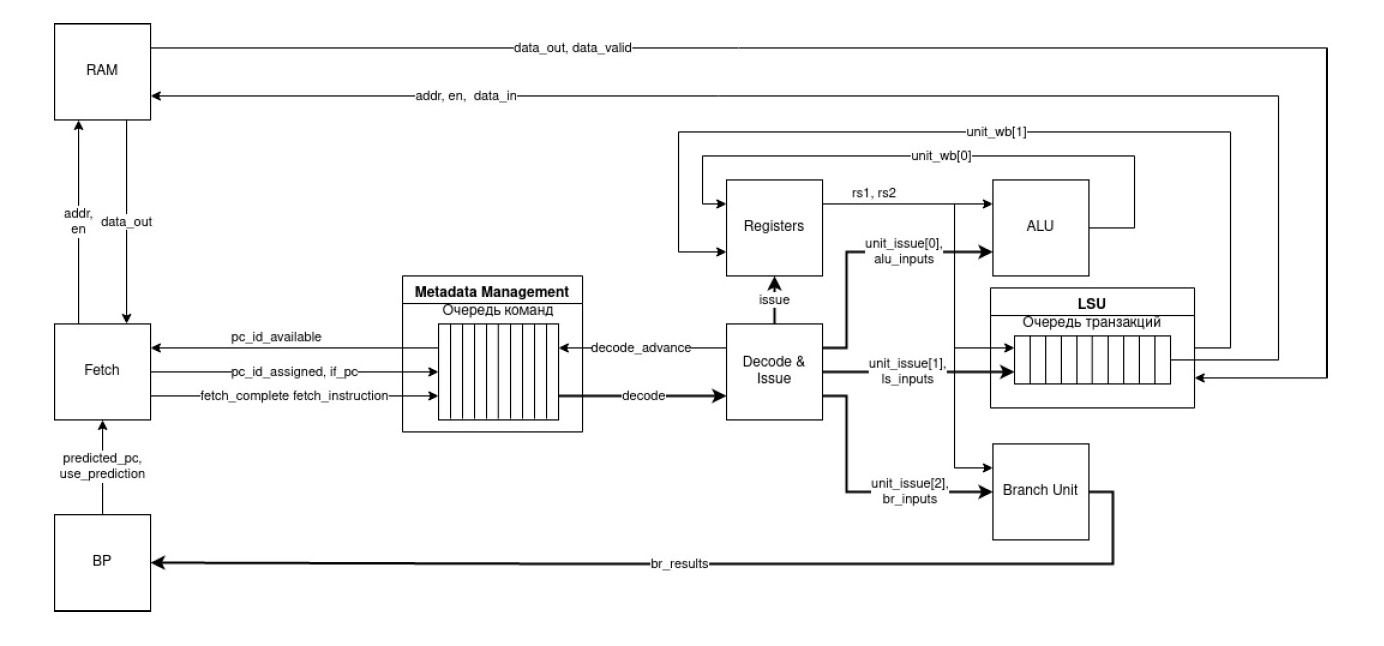
\includegraphics[scale=0.4]{taiga_scheme}}
	\caption{Обобщенная структурная схема ядра Taiga}
\end{figure}

\chapter{Практическая часть}

\section{Задание 1}

\begin{lstlisting}[label=some-code-1,caption=Листинг исходной программы]
    .section .text
    .globl _start;
    len = 8 #Размер массива
    enroll = 1 #Количество обрабатываемых элементов за одну итерацию
    elem_sz = 4 #Размер одного элемента массива

_start:
    addi x20, x0, len/enroll
    la x1, _x
lp:
    lw x2, 0(x1)
    addi x1, x1, elem_sz*enroll
    addi x20, x20, -1
    add x31, x31, x2 #!
    bne x20, x0, lp
    addi x31, x31, 1
lp2: j lp2

    .section .data
_x: .4byte 0x1
    .4byte 0x2
    .4byte 0x3
    .4byte 0x4
    .4byte 0x5
    .4byte 0x6
    .4byte 0x7
    .4byte 0x8
\end{lstlisting}

\begin{lstlisting}[label=some-code-2,caption=Дизассемблированный истинг исходной программы]
SYMBOL TABLE:
80000000 l    d  .text  00000000 .text
80000028 l    d  .data  00000000 .data
00000000 l    df *ABS*  00000000 var_2.o
00000008 l       *ABS*  00000000 len
00000001 l       *ABS*  00000000 enroll
00000004 l       *ABS*  00000000 elem_sz
80000028 l       .data  00000000 _x
8000000c l       .text  00000000 lp
80000024 l       .text  00000000 lp2
80000000 g       .text  00000000 _start
80000048 g       .data  00000000 _end



Disassembly of section .text:

80000000 <_start>:
80000000:       00800a13                addi    x20,x0,8
80000004:       00000097                auipc   x1,0x0
80000008:       02408093                addi    x1,x1,36 # 80000028 <_x>

8000000c <lp>:
8000000c:       0000a103                lw      x2,0(x1)
80000010:       00408093                addi    x1,x1,4
80000014:       fffa0a13                addi    x20,x20,-1
80000018:       002f8fb3                add     x31,x31,x2
8000001c:       fe0a18e3                bne     x20,x0,8000000c <lp>
80000020:       001f8f93                addi    x31,x31,1

80000024 <lp2>:
80000024:       0000006f                jal     x0,80000024 <lp2>

Disassembly of section .data:

80000028 <_x>:
80000028:       0001                    c.addi  x0,0
8000002a:       0000                    unimp
8000002c:       0002                    0x2
8000002e:       0000                    unimp
80000030:       00000003                lb      x0,0(x0) # 0 <enroll-0x1>
80000034:       0004                    c.addi4spn      x9,x2,0
80000036:       0000                    unimp
80000038:       0005                    c.addi  x0,1
8000003a:       0000                    unimp
8000003c:       0006                    0x6
8000003e:       0000                    unimp
80000040:       00000007                0x7
80000044:       0008                    c.addi4spn      x10,x2,0
\end{lstlisting}

\begin{lstlisting}[label=some-code-3,caption=Псевдокод на языке C эквивалентной программы]
#define len 8
#define enroll 1
#define elem_sz 4

int _x [] = {1, 2, 3, 4, 5, 6, 7, 8};
int x2, x3, x4, x5, x31;

void _start()
{
    int x_20 = len;
    int x1 [] = _x;

    do
    {
        x2 = x1[0];
        x1 += elem_sz * enroll;
        x20--;
        x31 += x2;
    } while (x20 != 0);
    x31++;

    while (1) {};
}
\end{lstlisting}

В результате выполнения данного кода в регистр x31 будет занесена инкрементированная сумма элементов массива, т.е. значение 0x25.

\section{Задание 2}
В задании 2 нужно найти такт, в котором выполняется выборка команды с адресом 80000010. То есть, в такте 5 команда добавляется в таблицу команд c\_abe. После этого в конце этого же такта ей присваивается значение d = 4. В 16 такте заканчивается этап декодирования, и код операции добавляется в таблицу c\_abe.

Рисунок диаграммы приведён ниже:
\begin{figure}[ph!]
	\center{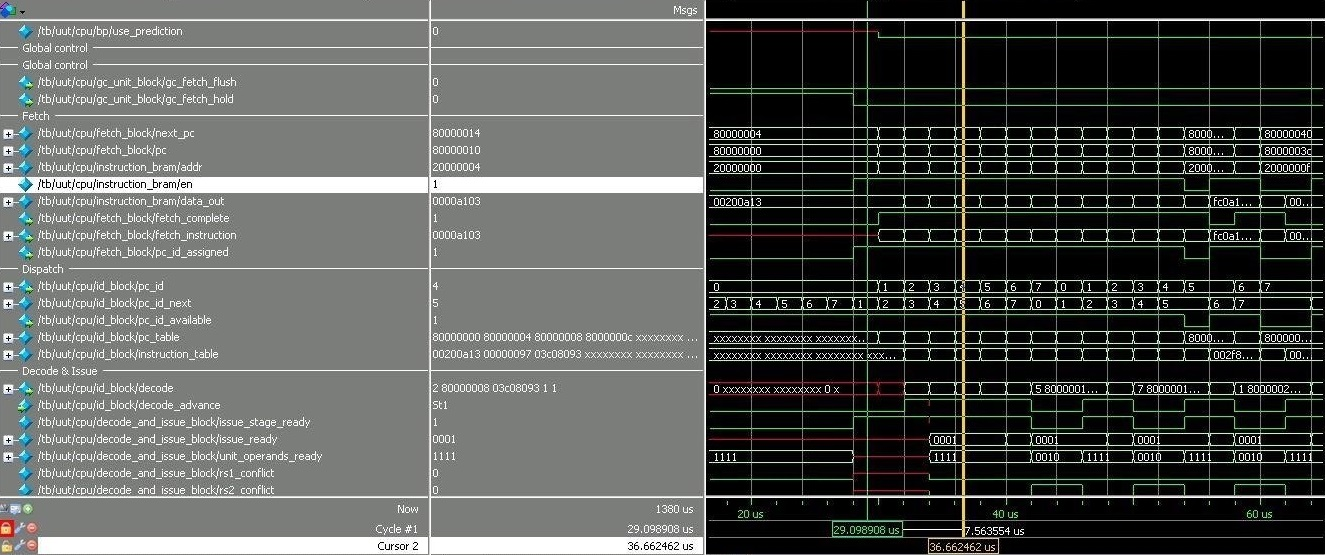
\includegraphics[scale=0.7]{task_1_diag}}
	\caption{Диаграмма, соответствующая этапам выборки и диспетчеризации}
\end{figure}

\section{Задание 3}
В задании 3 необходимо найти такт, в котором выполняется декодирование и планирование команды с адресом 8000001с. Результат декодирования мы можем увидеть в конце такта 14 - выполнение команды делегируется блоку доступа к памяти.

Рисунок диаграммы приведён ниже:
\begin{figure}[ph!]
	\center{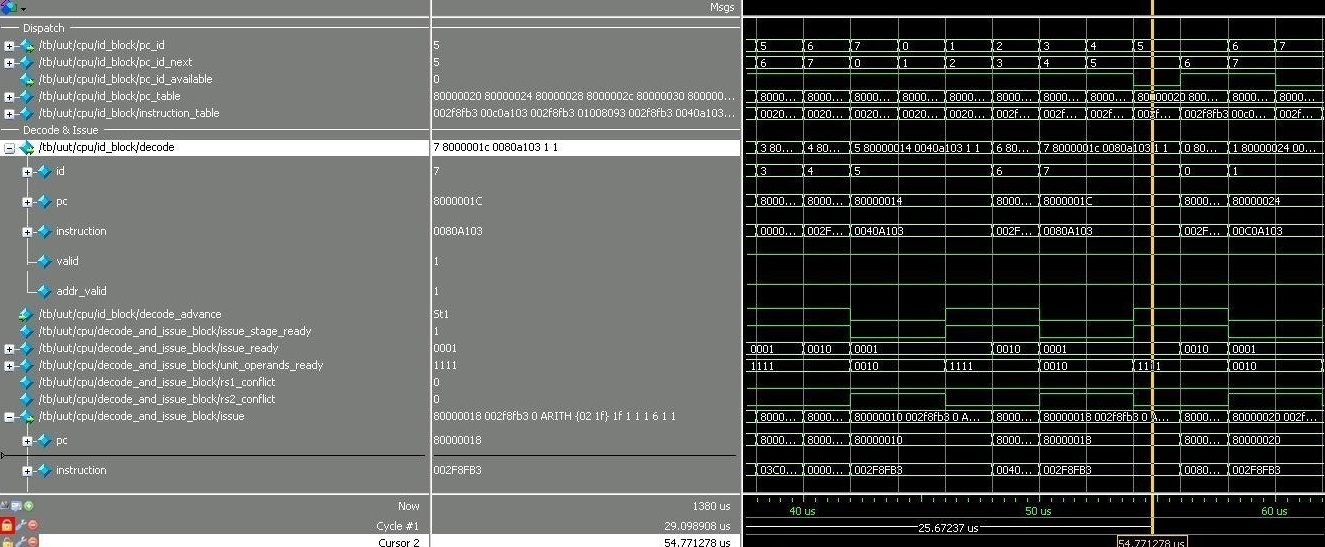
\includegraphics[scale=0.7]{task_2_diag}}
	\caption{Диаграмма, соответствующая этапам декодирования и планирования}
\end{figure}

\section{Задание 4}
В задании 4 выполняем поиск такта, в котором выполняется исполнение команды с адресом 80000004. 

Диаграмма, соответствующая этапу выполнения:

\begin{figure}[ph!]
	\center{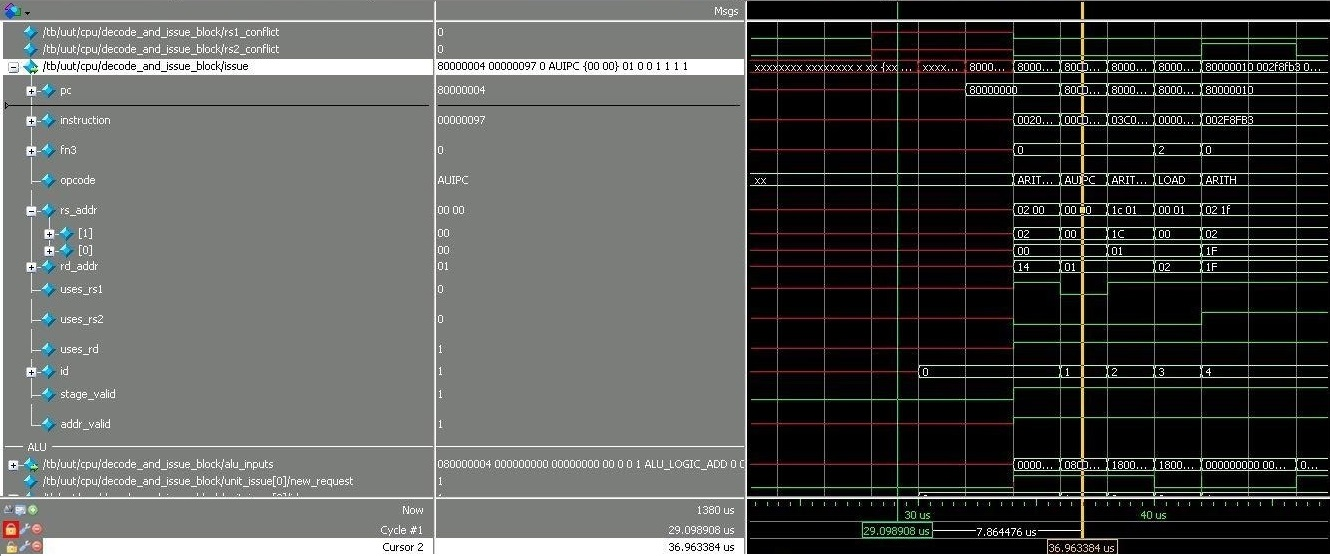
\includegraphics[scale=0.7]{task_3_diag}}
	\caption{Диаграмма, соответствующая этапам декодирования и планирования}
\end{figure}

\newpage

Результат выполнения программы заносится в регистр х31. В задании номер 1 было предсказано, что в нём хранится значение 0x25, что и видно на представленной ниже диаграмме.

\begin{figure}[ph!]
	\center{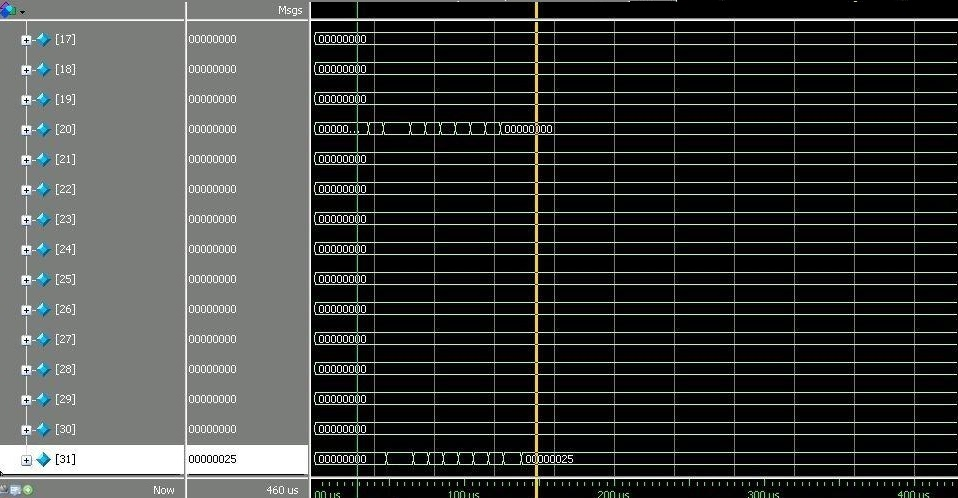
\includegraphics[scale=0.7]{task_4_diag}}
	\caption{Диаграмма, соответствующая этапам декодирования и планирования}
\end{figure}

\section{Задание 5}

В соответствие с заданием 5 мы должны рассмотреть порядок выполнения стадий конвейера процессора. Мы можем это сделать с помощью диаграммы трассы работы программы, которая приведена ниже.

\begin{figure}[ph!]
	\center{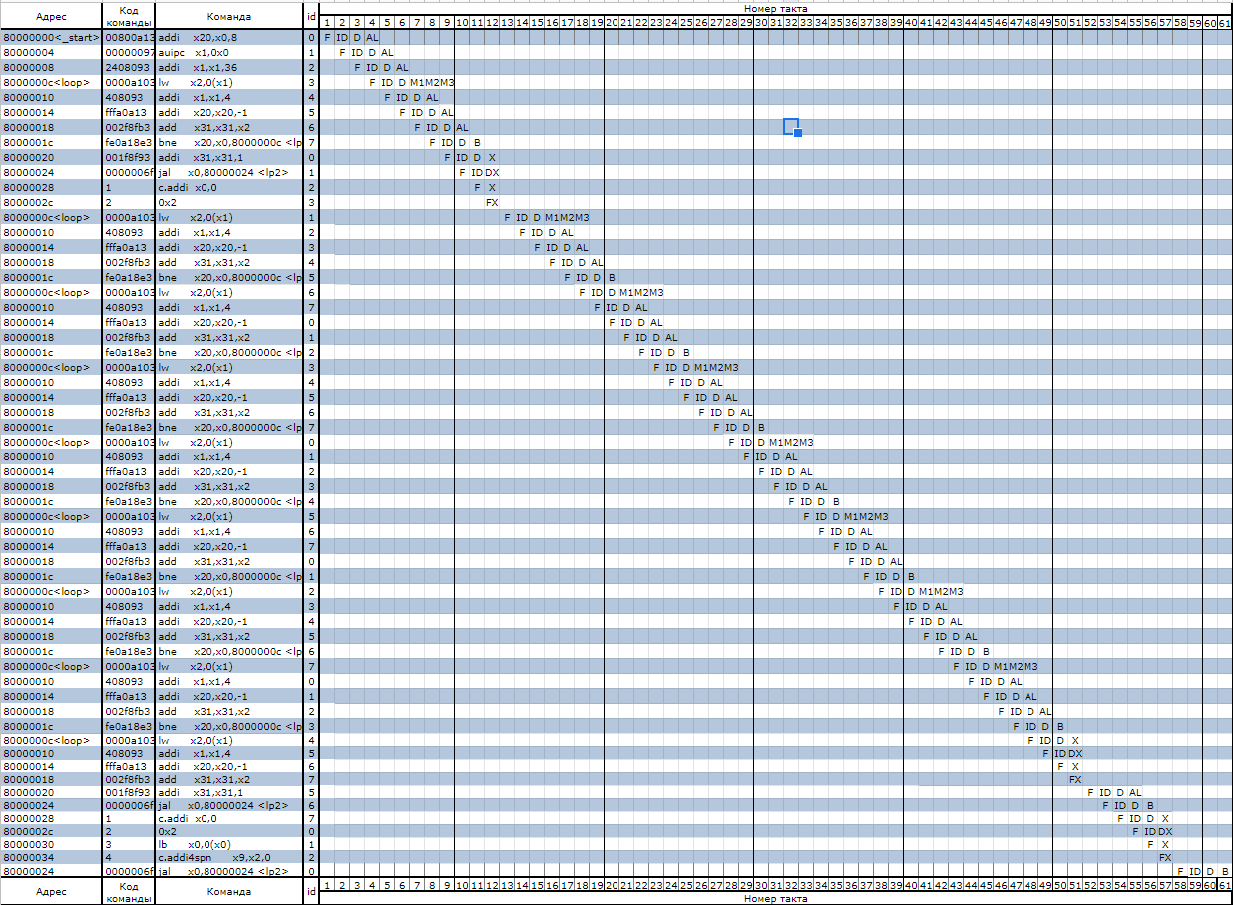
\includegraphics[scale=0.7]{trace}}
	\caption{Трасса работы программы}
\end{figure}

Ниже приведена диаграмма, поясняющая этапы обработки команды add x31, x31, x2\#!.

\newpage

\begin{figure}[ph!]
	\center{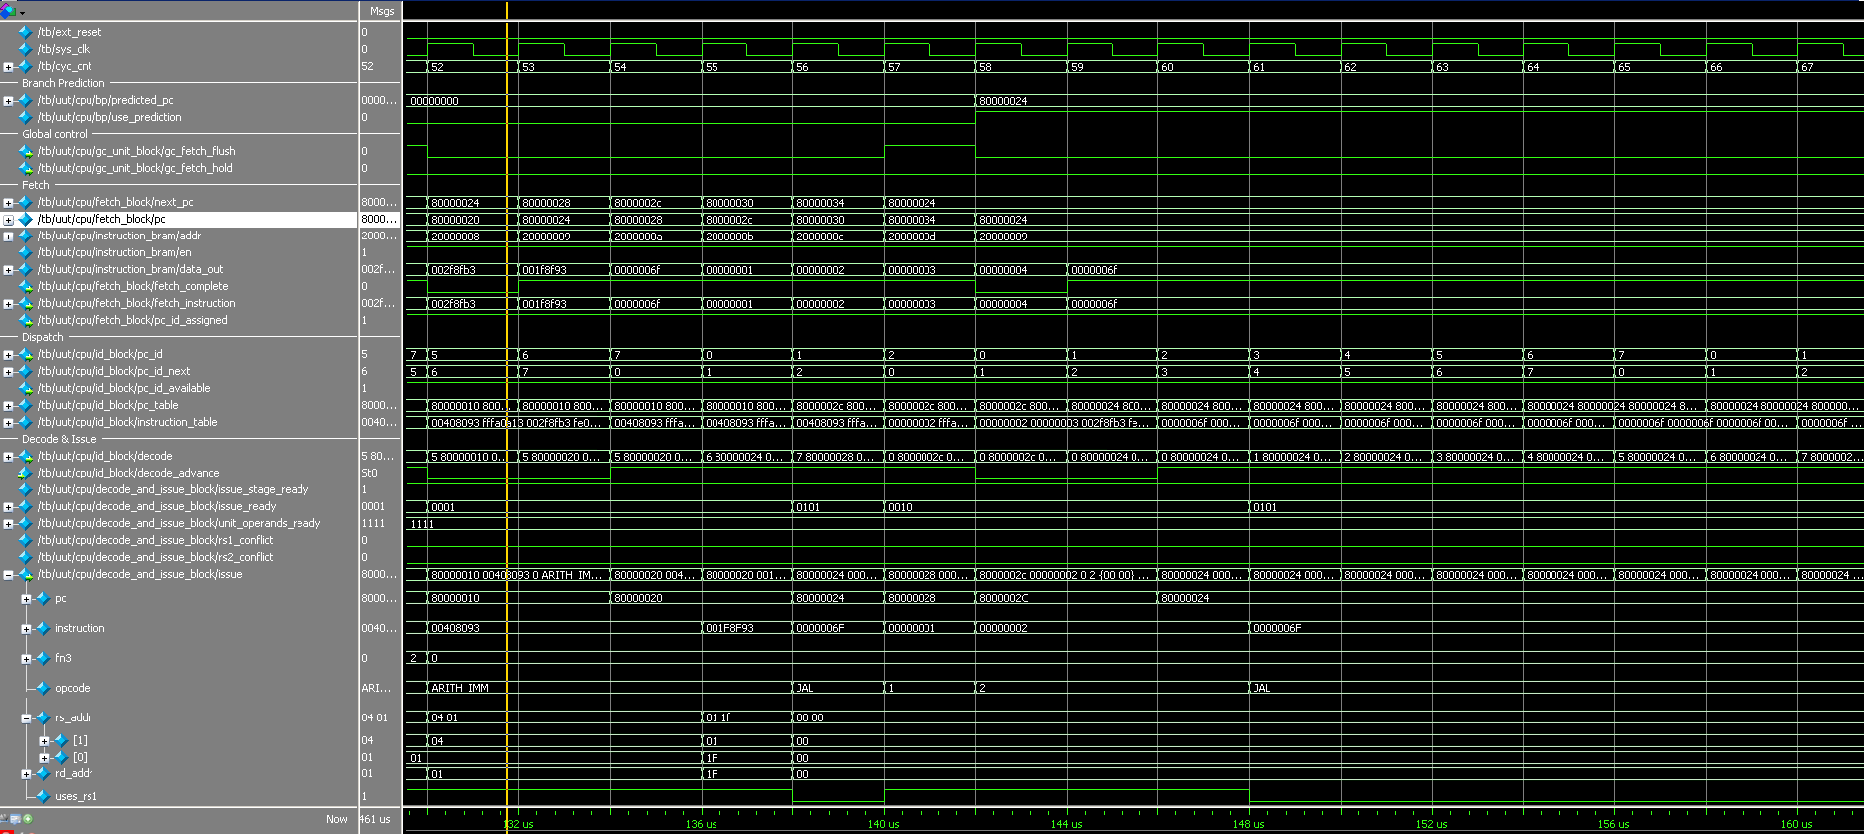
\includegraphics[scale=0.4]{comand_process}}
	\caption{Диаграмма, поясняющая обработку команды}
\end{figure}

Нужный нам адрес равен 80000020, данной команде на такте 53 присваивается pc\_id = 5. Декодирование выполняеся на 54 такте. Этап выполнения происходит на 55 такте.

Из выше представленной трассы видно, что во время выполнения программы не произошло конфликтов. Следовательно отсутствует возможность сократить время выполнения путем перестановки команд для ликвидации конфликтов.

Следовательно выполняемая программа имеет оптимальный порядок команд и не нуждается в оптимизации.

\chapter{Вывод}
В данной лабораторной работе было проведено ознакомление с архитектурой ядра Taiga, а именно с порядком работы вычислительного конвейера: изучены команды RV32I, рассмотрены действия, выполняемые на каждой стадии конвейера, и данные, передаваемые между ними. После ознакомления с теоретической стороной вопроса, был выполнен разбор этапов выполнения программы на симуляции процессора с набором инструкций RV32I. После ее анализа были сделаны выводы, что оптимизация не требуется. В итоге, теоретические знания о порядке исполнения программ на процессорах с RISC архитектурой были закреплены на практике. Таким образом все поставленные задачи решены, основная цель работы достигнута.
